\documentclass[tikz,border=5pt]{standalone}
\usepackage{ctex,amsmath}
\usetikzlibrary{arrows.meta,calc,patterns}
\tikzset{>=Latex,axis/.style={gray,->},electric/.style={blue!65!black,thick},force/.style={orange!85!black,very thick,->}}
\newcommand{\groundat}[2]{\draw (#1,#2)--++(0,-.25) ++(-.22,0)--++(.44,0) ++(-.36,-.10)--++(.28,0) ++(-.22,-.10)--++(.16,0);}
\begin{document}
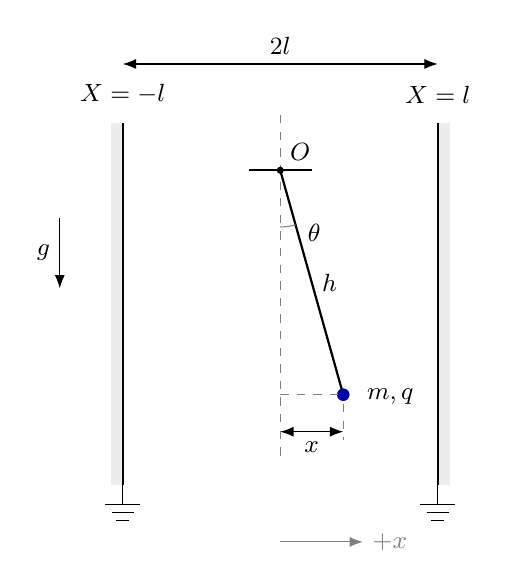
\begin{tikzpicture}[font=\small]
\fill[gray!15](-2.15,.6)rectangle(-2,-4.0);
\fill[gray!15](2,.6)rectangle(2.15,-4.0);
\draw[thick](-2,.6)--(-2,-4.0)(2,.6)--(2,-4.0);
\groundat{-2}{-4.0}\groundat{2}{-4.0}
\node[above]at(-2,.72){$X=-l$};\node[above]at(2,.72){$X=l$};
\draw[gray,dashed](0,.7)--(0,-3.65);
\draw[thick](-.40,0)--(.40,0);
\fill(0,0)circle[radius=.045]node[above right]{$O$};
\coordinate(Q)at(.80,-2.85);
\draw[thick](0,0)--(Q)node[midway,right]{$h$};
\fill[electric](Q)circle[radius=.08];
\node[right]at(.98,-2.88){$m,q$};
\draw[gray](0,-.72)arc[start angle=-90,end angle=-74.32,radius=.72];
\node at(.43,-.80){$\theta$};
\draw[gray,dashed](0,-2.85)--(Q);
\draw[<->](0,-3.32)--(.80,-3.32)node[midway,below]{$x$};
\draw[gray,dashed](.80,-2.97)--(.80,-3.42);
\draw[<->](-2,1.35)--(2,1.35)node[midway,above]{$2l$};
\draw[axis](0,-4.72)--(1.05,-4.72)node[right]{$+x$};
\draw[->](-2.8,-.6)--(-2.8,-1.5)node[midway,left]{$g$};
\end{tikzpicture}
\begin{tikzpicture}[font=\small,x=.72cm]
\fill[blue!5](-1,-.70)rectangle(1,.70);
\draw[gray,thick](-1,-.7)--(-1,.7)(1,-.7)--(1,.7);
\node[above]at(-1,.75){$-l$};\node[above]at(1,.75){$l$};
\draw[axis](-7.15,0)--(6.85,0)node[right]{$X$};
\foreach \xx in {-6.2,-2.2,1.8,5.8}{\draw[red!65!black,thick](\xx,0)circle[radius=.08];\node[above]at(\xx,.12){$-q$};}
\foreach \xx in {-3.8,4.2}{\draw[blue!65!black,thick](\xx,0)circle[radius=.08];\node[above]at(\xx,.12){$+q$};}
\fill[black](.2,0)circle[radius=.075];\node[above]at(.2,.14){$q$};
\node[below]at(-6.2,-.62){$-6l-x$};
\node[below]at(-3.8,-.18){$x-4l$};
\node[below]at(-2.2,-.62){$-2l-x$};
\node[below]at(.2,-.18){$x$};
\node[below]at(1.8,-.62){$2l-x$};
\node[below]at(4.2,-.18){$x+4l$};
\node[below]at(5.8,-.62){$6l-x$};
\node at(-7,.25){$\cdots$};\node at(6.7,.25){$\cdots$};
\node[below]at(0,-1.35){浅色区域：两板之间};
\end{tikzpicture}
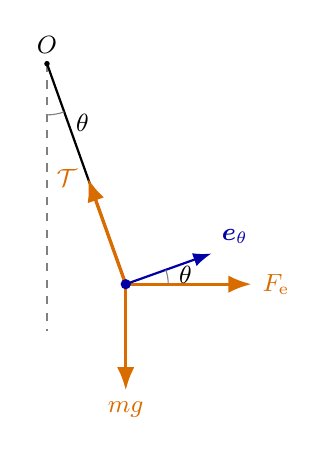
\begin{tikzpicture}[font=\small]
\coordinate(O)at(0,0);\coordinate(Q)at(1,-2.8);
\draw[gray,dashed](O)--(0,-3.4);
\draw[thick](O)--(Q);\fill(O)circle[radius=.035]node[above]{$O$};
\draw[gray](0,-.65)arc[start angle=-90,end angle=-70.35,radius=.65];
\node at(.45,-.75){$\theta$};
\draw[force](Q)--(.52,-1.456)node[left]{$\mathcal T$};
\draw[force](Q)--(1,-4.15)node[below]{$mg$};
\draw[force](Q)--(2.6,-2.8)node[right]{$F_{\mathrm e}$};
\draw[blue!65!black,thick,->](Q)--(2.09,-2.41)node[above right]{$\boldsymbol e_\theta$};
\fill[blue!65!black](Q)circle[radius=.065];
\draw[gray](1.54,-2.8)arc[start angle=0,end angle=19.65,radius=.54];
\node at(1.76,-2.68){$\theta$};
\end{tikzpicture}
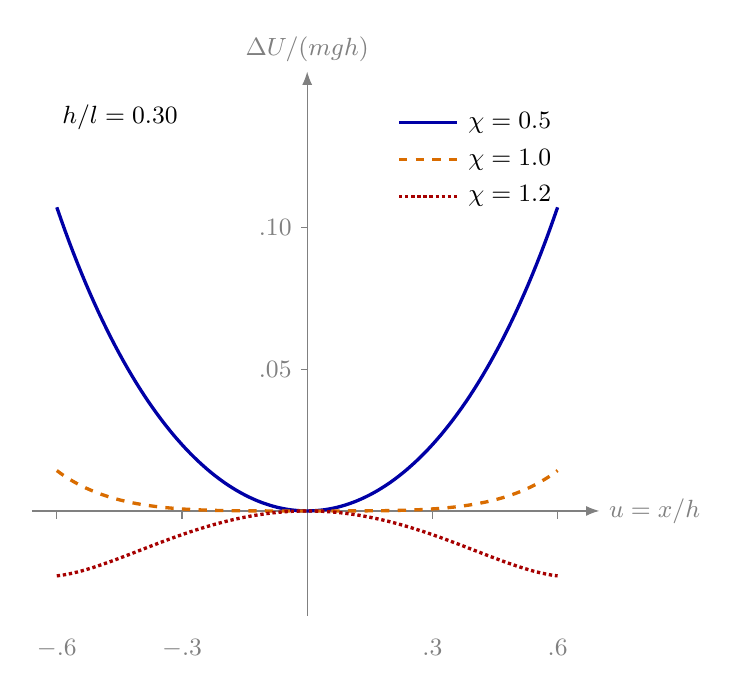
\begin{tikzpicture}[font=\small,x=5.3cm,y=36cm]
\draw[axis](-.66,0)--(.70,0)node[right]{$u=x/h$};
\draw[axis](0,-.037)--(0,.155)node[above]{$\Delta U/(mgh)$};
\foreach \t in {-.6,-.3,.3,.6}{\draw[gray](\t,0)--(\t,-.003);\node[below,gray]at(\t,-.042){$\t$};}
\foreach \t in {.05,.10}\draw[gray](0,\t)--(-.014,\t)node[left]{$\t$};
\draw[blue!65!black,very thick,solid] plot coordinates {(-0.600000,0.1071221922) (-0.590000,0.1028840211) (-0.580000,0.0987761455) (-0.570000,0.0947939133) (-0.560000,0.0909329604) (-0.550000,0.0871891883) (-0.540000,0.0835587436) (-0.530000,0.0800379995) (-0.520000,0.0766235394) (-0.510000,0.0733121415) (-0.500000,0.0701007652) (-0.490000,0.0669865386) (-0.480000,0.0639667470) (-0.470000,0.0610388228) (-0.460000,0.0582003356) (-0.450000,0.0554489839) (-0.440000,0.0527825864) (-0.430000,0.0501990756) (-0.420000,0.0476964902) (-0.410000,0.0452729692) (-0.400000,0.0429267462) (-0.390000,0.0406561440) (-0.380000,0.0384595697) (-0.370000,0.0363355100) (-0.360000,0.0342825274) (-0.350000,0.0322992556) (-0.340000,0.0303843967) (-0.330000,0.0285367172) (-0.320000,0.0267550450) (-0.310000,0.0250382667) (-0.300000,0.0233853247) (-0.290000,0.0217952149) (-0.280000,0.0202669838) (-0.270000,0.0187997271) (-0.260000,0.0173925869) (-0.250000,0.0160447504) (-0.240000,0.0147554478) (-0.230000,0.0135239506) (-0.220000,0.0123495703) (-0.210000,0.0112316569) (-0.200000,0.0101695973) (-0.190000,0.0091628145) (-0.180000,0.0082107662) (-0.170000,0.0073129435) (-0.160000,0.0064688705) (-0.150000,0.0056781027) (-0.140000,0.0049402268) (-0.130000,0.0042548595) (-0.120000,0.0036216467) (-0.110000,0.0030402633) (-0.100000,0.0025104121) (-0.090000,0.0020318237) (-0.080000,0.0016042558) (-0.070000,0.0012274925) (-0.060000,0.0009013443) (-0.050000,0.0006256479) (-0.040000,0.0004002652) (-0.030000,0.0002250839) (-0.020000,0.0001000166) (-0.010000,0.0000250010) (0.000000,0.0000000000) (0.010000,0.0000250010) (0.020000,0.0001000166) (0.030000,0.0002250839) (0.040000,0.0004002652) (0.050000,0.0006256479) (0.060000,0.0009013443) (0.070000,0.0012274925) (0.080000,0.0016042558) (0.090000,0.0020318237) (0.100000,0.0025104121) (0.110000,0.0030402633) (0.120000,0.0036216467) (0.130000,0.0042548595) (0.140000,0.0049402268) (0.150000,0.0056781027) (0.160000,0.0064688705) (0.170000,0.0073129435) (0.180000,0.0082107662) (0.190000,0.0091628145) (0.200000,0.0101695973) (0.210000,0.0112316569) (0.220000,0.0123495703) (0.230000,0.0135239506) (0.240000,0.0147554478) (0.250000,0.0160447504) (0.260000,0.0173925869) (0.270000,0.0187997271) (0.280000,0.0202669838) (0.290000,0.0217952149) (0.300000,0.0233853247) (0.310000,0.0250382667) (0.320000,0.0267550450) (0.330000,0.0285367172) (0.340000,0.0303843967) (0.350000,0.0322992556) (0.360000,0.0342825274) (0.370000,0.0363355100) (0.380000,0.0384595697) (0.390000,0.0406561440) (0.400000,0.0429267462) (0.410000,0.0452729692) (0.420000,0.0476964902) (0.430000,0.0501990756) (0.440000,0.0527825864) (0.450000,0.0554489839) (0.460000,0.0582003356) (0.470000,0.0610388228) (0.480000,0.0639667470) (0.490000,0.0669865386) (0.500000,0.0701007652) (0.510000,0.0733121415) (0.520000,0.0766235394) (0.530000,0.0800379995) (0.540000,0.0835587436) (0.550000,0.0871891883) (0.560000,0.0909329604) (0.570000,0.0947939133) (0.580000,0.0987761455) (0.590000,0.1028840211) (0.600000,0.1071221922)};
\draw[orange!85!black,very thick,dashed] plot coordinates {(-0.600000,0.0142443844) (-0.590000,0.0131712871) (-0.580000,0.0121687651) (-0.570000,0.0112325186) (-0.560000,0.0103585278) (-0.550000,0.0095430310) (-0.540000,0.0087825036) (-0.530000,0.0080736405) (-0.520000,0.0074133390) (-0.510000,0.0067986840) (-0.500000,0.0062269342) (-0.490000,0.0056955100) (-0.480000,0.0052019819) (-0.470000,0.0047440605) (-0.460000,0.0043195865) (-0.450000,0.0039265227) (-0.440000,0.0035629457) (-0.430000,0.0032270387) (-0.420000,0.0029170847) (-0.410000,0.0026314607) (-0.400000,0.0023686314) (-0.390000,0.0021271446) (-0.380000,0.0019056258) (-0.370000,0.0017027741) (-0.360000,0.0015173579) (-0.350000,0.0013482110) (-0.340000,0.0011942291) (-0.330000,0.0010543663) (-0.320000,0.0009276325) (-0.310000,0.0008130899) (-0.300000,0.0007098509) (-0.290000,0.0006170752) (-0.280000,0.0005339677) (-0.270000,0.0004597764) (-0.260000,0.0003937902) (-0.250000,0.0003353374) (-0.240000,0.0002837836) (-0.230000,0.0002385300) (-0.220000,0.0001990125) (-0.210000,0.0001646997) (-0.200000,0.0001350918) (-0.190000,0.0001097194) (-0.180000,0.0000881426) (-0.170000,0.0000699494) (-0.160000,0.0000547553) (-0.150000,0.0000422021) (-0.140000,0.0000319572) (-0.130000,0.0000237128) (-0.120000,0.0000171850) (-0.110000,0.0000121137) (-0.100000,0.0000082613) (-0.090000,0.0000054129) (-0.080000,0.0000033751) (-0.070000,0.0000019763) (-0.060000,0.0000010658) (-0.050000,0.0000005136) (-0.040000,0.0000002102) (-0.030000,0.0000000665) (-0.020000,0.0000000131) (-0.010000,0.0000000008) (0.000000,0.0000000000) (0.010000,0.0000000008) (0.020000,0.0000000131) (0.030000,0.0000000665) (0.040000,0.0000002102) (0.050000,0.0000005136) (0.060000,0.0000010658) (0.070000,0.0000019763) (0.080000,0.0000033751) (0.090000,0.0000054129) (0.100000,0.0000082613) (0.110000,0.0000121137) (0.120000,0.0000171850) (0.130000,0.0000237128) (0.140000,0.0000319572) (0.150000,0.0000422021) (0.160000,0.0000547553) (0.170000,0.0000699494) (0.180000,0.0000881426) (0.190000,0.0001097194) (0.200000,0.0001350918) (0.210000,0.0001646997) (0.220000,0.0001990125) (0.230000,0.0002385300) (0.240000,0.0002837836) (0.250000,0.0003353374) (0.260000,0.0003937902) (0.270000,0.0004597764) (0.280000,0.0005339677) (0.290000,0.0006170752) (0.300000,0.0007098509) (0.310000,0.0008130899) (0.320000,0.0009276325) (0.330000,0.0010543663) (0.340000,0.0011942291) (0.350000,0.0013482110) (0.360000,0.0015173579) (0.370000,0.0017027741) (0.380000,0.0019056258) (0.390000,0.0021271446) (0.400000,0.0023686314) (0.410000,0.0026314607) (0.420000,0.0029170847) (0.430000,0.0032270387) (0.440000,0.0035629457) (0.450000,0.0039265227) (0.460000,0.0043195865) (0.470000,0.0047440605) (0.480000,0.0052019819) (0.490000,0.0056955100) (0.500000,0.0062269342) (0.510000,0.0067986840) (0.520000,0.0074133390) (0.530000,0.0080736405) (0.540000,0.0087825036) (0.550000,0.0095430310) (0.560000,0.0103585278) (0.570000,0.0112325186) (0.580000,0.0121687651) (0.590000,0.0131712871) (0.600000,0.0142443844)};
\draw[red!65!black,very thick,densely dotted] plot coordinates {(-0.600000,-0.0229067387) (-0.590000,-0.0227138065) (-0.580000,-0.0224741870) (-0.570000,-0.0221920393) (-0.560000,-0.0218712452) (-0.550000,-0.0215154320) (-0.540000,-0.0211279924) (-0.530000,-0.0207121031) (-0.520000,-0.0202707412) (-0.510000,-0.0198066991) (-0.500000,-0.0193225982) (-0.490000,-0.0188209014) (-0.480000,-0.0183039241) (-0.470000,-0.0177738444) (-0.460000,-0.0172327131) (-0.450000,-0.0166824617) (-0.440000,-0.0161249106) (-0.430000,-0.0155617761) (-0.420000,-0.0149946774) (-0.410000,-0.0144251427) (-0.400000,-0.0138546145) (-0.390000,-0.0132844552) (-0.380000,-0.0127159518) (-0.370000,-0.0121503203) (-0.360000,-0.0115887099) (-0.350000,-0.0110322068) (-0.340000,-0.0104818380) (-0.330000,-0.0099385740) (-0.320000,-0.0094033325) (-0.310000,-0.0088769808) (-0.300000,-0.0083603386) (-0.290000,-0.0078541807) (-0.280000,-0.0073592388) (-0.270000,-0.0068762039) (-0.260000,-0.0064057284) (-0.250000,-0.0059484278) (-0.240000,-0.0055048821) (-0.230000,-0.0050756382) (-0.220000,-0.0046612106) (-0.210000,-0.0042620832) (-0.200000,-0.0038787105) (-0.190000,-0.0035115186) (-0.180000,-0.0031609069) (-0.170000,-0.0028272483) (-0.160000,-0.0025108908) (-0.150000,-0.0022121581) (-0.140000,-0.0019313506) (-0.130000,-0.0016687459) (-0.120000,-0.0014245996) (-0.110000,-0.0011991461) (-0.100000,-0.0009925990) (-0.090000,-0.0008051515) (-0.080000,-0.0006369772) (-0.070000,-0.0004882302) (-0.060000,-0.0003590457) (-0.050000,-0.0002495402) (-0.040000,-0.0001598118) (-0.030000,-0.0000899405) (-0.020000,-0.0000399882) (-0.010000,-0.0000099993) (0.000000,0.0000000000) (0.010000,-0.0000099993) (0.020000,-0.0000399882) (0.030000,-0.0000899405) (0.040000,-0.0001598118) (0.050000,-0.0002495402) (0.060000,-0.0003590457) (0.070000,-0.0004882302) (0.080000,-0.0006369772) (0.090000,-0.0008051515) (0.100000,-0.0009925990) (0.110000,-0.0011991461) (0.120000,-0.0014245996) (0.130000,-0.0016687459) (0.140000,-0.0019313506) (0.150000,-0.0022121581) (0.160000,-0.0025108908) (0.170000,-0.0028272483) (0.180000,-0.0031609069) (0.190000,-0.0035115186) (0.200000,-0.0038787105) (0.210000,-0.0042620832) (0.220000,-0.0046612106) (0.230000,-0.0050756382) (0.240000,-0.0055048821) (0.250000,-0.0059484278) (0.260000,-0.0064057284) (0.270000,-0.0068762039) (0.280000,-0.0073592388) (0.290000,-0.0078541807) (0.300000,-0.0083603386) (0.310000,-0.0088769808) (0.320000,-0.0094033325) (0.330000,-0.0099385740) (0.340000,-0.0104818380) (0.350000,-0.0110322068) (0.360000,-0.0115887099) (0.370000,-0.0121503203) (0.380000,-0.0127159518) (0.390000,-0.0132844552) (0.400000,-0.0138546145) (0.410000,-0.0144251427) (0.420000,-0.0149946774) (0.430000,-0.0155617761) (0.440000,-0.0161249106) (0.450000,-0.0166824617) (0.460000,-0.0172327131) (0.470000,-0.0177738444) (0.480000,-0.0183039241) (0.490000,-0.0188209014) (0.500000,-0.0193225982) (0.510000,-0.0198066991) (0.520000,-0.0202707412) (0.530000,-0.0207121031) (0.540000,-0.0211279924) (0.550000,-0.0215154320) (0.560000,-0.0218712452) (0.570000,-0.0221920393) (0.580000,-0.0224741870) (0.590000,-0.0227138065) (0.600000,-0.0229067387)};

\draw[blue!65!black,very thick](.22,.137)--(.36,.137)node[right,black]{$\chi=0.5$};
\draw[orange!85!black,very thick,dashed](.22,.124)--(.36,.124)node[right,black]{$\chi=1.0$};
\draw[red!65!black,very thick,densely dotted](.22,.111)--(.36,.111)node[right,black]{$\chi=1.2$};
\node[anchor=west]at(-.61,.139){$h/l=0.30$};
\end{tikzpicture}
\end{document}
